%!Mode:: "TeX:UTF-8"
\documentclass[a4paper,11pt,UTF8]{ctexart}

\usepackage{indentfirst} %缩进
\usepackage{xeCJK}    %使用系统字体
\usepackage{fancyhdr} %自定义页眉页脚
\pagestyle{empty}                   %不设置页眉页脚
\usepackage{amsmath, amsthm, amssymb, amsfonts} %数学公式
\usepackage[a4paper,left=3cm,right=3cm,top=3cm,bottom=3cm]{geometry}
%\usepackage[tmargin=1in,bmargin=1in,lmargin=1.25in,rmargin=1.25in]{geometry}.
\usepackage{booktabs} %插入表格
\usepackage[section]{placeins} %避免浮动
\usepackage{listings} %插入代码
\usepackage{ctex}     %中文宏包
\usepackage[svgnames, table]{xcolor} %彩色表格
\usepackage{algorithm}          %伪代码
\usepackage{algorithmicx}
\usepackage{algpseudocode}
\usepackage{algorithm,algpseudocode,float}
\usepackage{lipsum}
\usepackage{enumitem}           %调整列举环境
\usepackage{url}
\usepackage{fontspec,xunicode}
\usepackage{subfigure}
\usepackage{parskip}      %m行n列图片排版方法
\defaultfontfeatures{Mapping=tex-text} %如果没有它,会有一些 tex 特殊字符无法正常使用,比如连字符。

\usepackage{graphicx}
\graphicspath{{imgs/}}

%%%%%%%%%%%%%%%%%%%%%%%%%%%%%%%%%%%%%%%%%%%%%%%%%%%%%%%%%%%%%%%%
% 缩进及行间距
%%%%%%%%%%%%%%%%%%%%%%%%%%%%%%%%%%%%%%%%%%%%%%%%%%%%%%%%%%%%%%%%
\setlength{\parindent}{22pt} %重新定义缩进长度
\setlength{\baselineskip}{20pt}  %定义行间距
%\renewcommand{\baselinestretch}{1.1} %定义行间距

%%%%%%%%%%%%%%%%%%%%%%%%%%%%%%%%%%%%%%%%%%%%%%%%%%%%%%%%%%%%%%%%
% 列表设置
%%%%%%%%%%%%%%%%%%%%%%%%%%%%%%%%%%%%%%%%%%%%%%%%%%%%%%%%%%%%%%%%
\setenumerate{fullwidth,itemindent=\parindent,listparindent=\parindent,itemsep=0ex,partopsep=0pt,parsep=0ex}
\setenumerate[2]{label=\alph*),leftmargin=1.5em}  %二级item设置
\setitemize{itemindent=38pt,leftmargin=0pt,itemsep=-0.4ex,listparindent=26pt,partopsep=0pt,parsep=0.5ex,topsep=-0.25ex}
\setdescription{itemindent=38pt,leftmargin=0pt,itemsep=-0.4ex,listparindent=26pt,partopsep=0pt,parsep=0.5ex,topsep=-0.25ex}

%%%%%%%%%%%%%%%%%%%%%%%%%%%%%%%%%%%%%%%%%%%%%%%%%%%%%%%%%%%%%%%%
% 图的标题行间距设置
%%%%%%%%%%%%%%%%%%%%%%%%%%%%%%%%%%%%%%%%%%%%%%%%%%%%%%%%%%%%%%%%
\newcommand{\bottomcaption}{%
\setlength{\abovecaptionskip}{6pt}%
\setlength{\belowcaptionskip}{6pt}%
\caption}


%%%%%%%%%%%%%%%%%%%%%%%%%%%%%%%%%%%%%%%%%%%%%%%%%%%%%%%%%%%%%%%%
% 字体定义
%%%%%%%%%%%%%%%%%%%%%%%%%%%%%%%%%%%%%%%%%%%%%%%%%%%%%%%%%%%%%%%%
\setmainfont{Times New Roman}  %默认英文字体.serif是有衬线字体sans serif无衬线字体
\setmonofont{FiraCode-Retina.ttf}
\setCJKmainfont[ItalicFont={楷体}, BoldFont={黑体}]{宋体}%衬线字体 缺省中文字体为
\setCJKsansfont{黑体}
\punctstyle{hangmobanjiao}
%-----------------------xeCJK下设置中文字体------------------------------%
\setCJKfamilyfont{song}{SimSun}                             %宋体 song
\newcommand{\song}{\CJKfamily{song}}
\setCJKfamilyfont{fs}{FangSong}                      %仿宋  fs
\newcommand{\fs}{\CJKfamily{fs}}
\setCJKfamilyfont{ktgb}{KaiTi}                      %楷体2312 ktgb
\newcommand{\ktgb}{\CJKfamily{ktgb}}
\setCJKfamilyfont{yh}{Microsoft YaHei}                    %微软雅黑 yh
\newcommand{\yh}{\CJKfamily{yh}}
\setCJKfamilyfont{hei}{SimHei}                              %黑体  hei
\newcommand{\hei}{\CJKfamily{hei}}
\setCJKfamilyfont{hwxk}{STXingkai}                                %华文行楷  hwxk
\newcommand{\hwxk}{\CJKfamily{hwxk}}
%------------------------------设置字体大小------------------------%
\newcommand{\shiyanbaogao}{\fontsize{36pt}{\baselineskip}\selectfont}
\newcommand{\chuhao}{\fontsize{42pt}{\baselineskip}\selectfont}     %初号
\newcommand{\xiaochuhao}{\fontsize{36pt}{\baselineskip}\selectfont} %小初号
\newcommand{\yihao}{\fontsize{28pt}{\baselineskip}\selectfont}      %一号
\newcommand{\erhao}{\fontsize{21pt}{\baselineskip}\selectfont}      %二号
\newcommand{\xiaoerhao}{\fontsize{18pt}{\baselineskip}\selectfont}  %小二号
\newcommand{\sanhao}{\fontsize{15.75pt}{\baselineskip}\selectfont}  %三号
\newcommand{\sihao}{\fontsize{14pt}{\baselineskip}\selectfont}       %四号
\newcommand{\xiaosihao}{\fontsize{12pt}{\baselineskip}\selectfont}  %小四号
\newcommand{\wuhao}{\fontsize{10.5pt}{\baselineskip}\selectfont}    %五号
\newcommand{\xiaowuhao}{\fontsize{9pt}{\baselineskip}\selectfont}   %小五号
\newcommand{\liuhao}{\fontsize{7.875pt}{\baselineskip}\selectfont}  %六号
\newcommand{\qihao}{\fontsize{5.25pt}{\baselineskip}\selectfont}    %七号

%%%%%%%%%%%%%%%%%%%%%%%%%%%%%%%%%%%%%%%%%%%%%%%%%%%%%%%%%%%%%%%%
% 图题字体大小相同
%%%%%%%%%%%%%%%%%%%%%%%%%%%%%%%%%%%%%%%%%%%%%%%%%%%%%%%%%%%%%%%%
\usepackage{caption}
\captionsetup{font={footnotesize}}   % footnotesize = 9pt
\captionsetup[lstlisting]{font={footnotesize}}

%%%%%%%%%%%%%%%%%%%%%%%%%%%%%%%%%%%%%%%%%%%%%%%%%%%%%%%%%%%%%%%%
% 重定义枚举编号为 1),2)...
%%%%%%%%%%%%%%%%%%%%%%%%%%%%%%%%%%%%%%%%%%%%%%%%%%%%%%%%%%%%%%%%
\renewcommand{\labelenumi}{\theenumi)}


%%%%%%%%%%%%%%%%%%%%%%%%%%%%%%%%%%%%%%%%%%%%%%%%%%%%%%%%%%%%%%%%
% 重定义section标题
%%%%%%%%%%%%%%%%%%%%%%%%%%%%%%%%%%%%%%%%%%%%%%%%%%%%%%%%%%%%%%%%
\CTEXsetup[format={\sihao\CJKfamily{zhhei}\zihao{4}},number={\chinese{section}},name={,、~},aftername={},indent={0pt},beforeskip={6pt},afterskip={6pt},format+={\flushleft}]{section}
\CTEXsetup[format={\Large\bfseries\CJKfamily{zhkai}\zihao{5}},name={(,)},number={\chinese{subsection}},aftername={},indent={22pt},beforeskip={14pt},afterskip={2pt}]{subsection}
\CTEXsetup[number={\chinese{section}},name={附录, ~~ }]{appendix}



%%%%%%%%%%%%%%%%%%%%%%%%%%%%%%%%%%%%%%%%%%%%%%%%%%%%%%%%%%%%%%%%
% 标题名称中文化
%%%%%%%%%%%%%%%%%%%%%%%%%%%%%%%%%%%%%%%%%%%%%%%%%%%%%%%%%%%%%%%%
\renewcommand\figurename{\hei 图}
\renewcommand\tablename{\hei 表}
\renewcommand\lstlistingname{\hei 代码}
\renewcommand{\algorithmicrequire}{\textbf{输入:}}
\renewcommand{\algorithmicensure}{\textbf{输出:}}
\newtheorem{define}{定义}

%%%%%%%%%%%%%%%%%%%%%%%%%%%%%%%%%%%%%%%%%%%%%%%%%%%%%%%%%%%%%%%%
% 代码设置
%%%%%%%%%%%%%%%%%%%%%%%%%%%%%%%%%%%%%%%%%%%%%%%%%%%%%%%%%%%%%%%%
\lstset{
 columns=fixed,
 numbers=left,                                        % 在左侧显示行号
 numberstyle=\tiny\color{gray},                       % 设定行号格式
 frame=single,                                      % 单线背景边框
%  frame=none,                                          % 不显示背景边框
 breaklines=true,                                     % 设定LaTeX对过长的代码行进行自动换行
 tabsize=4,                                           % 把tab扩展为4个空格,默认是8个太长
 keywordstyle=\color[RGB]{40,40,255},                 % 设定关键字颜色
 numberstyle=\footnotesize\color{darkgray}\ttfamily,
 commentstyle=\it\color[RGB]{0,96,96}\ttfamily,       % 设置代码注释的格式
 stringstyle=\rmfamily\slshape\color[RGB]{128,0,0},   % 设置字符串格式
 showstringspaces=false,                              % 不显示字符串中的空格
 language=c++,                                        % 设置语言
 basicstyle=\linespread{0.7}\xiaowuhao\ttfamily,                      % 字体字号
 morekeywords={alignas,continute,friend,register,true,alignof,decltype,goto,
 reinterpret_cast,try,asm,defult,if,return,typedef,auto,delete,inline,short,
 typeid,bool,do,int,signed,typename,break,double,long,sizeof,union,case,
 dynamic_cast,mutable,static,unsigned,catch,else,namespace,static_assert,using,
 char,enum,new,static_cast,virtual,char16_t,char32_t,explict,noexcept,struct,
 void,export,nullptr,switch,volatile,class,extern,operator,template,wchar_t,
 const,false,private,this,while,constexpr,float,protected,thread_local,
 const_cast,for,public,throw,std},
 xleftmargin=2em,
 xrightmargin=2em,
 aboveskip=1em
 %lineskip=10pt,
 %baselinestretch=1,
}

%%%%%%%%%%%%%%%%%%%%%%%%%%%%%%%%%%%%%%%%%%%%%%%%%%%%%%%%%%%%%%%%
% 伪代码分页
%%%%%%%%%%%%%%%%%%%%%%%%%%%%%%%%%%%%%%%%%%%%%%%%%%%%%%%%%%%%%%%%
\makeatletter
\renewcommand{\ALG@name}{算法}
\newenvironment{breakablealgorithm}
  {% \begin{breakablealgorithm}
   \begin{center}
     \refstepcounter{algorithm}% New algorithm
     \hrule height.8pt depth0pt \kern2pt% \@fs@pre for \@fs@ruled
     \renewcommand{\caption}[2][\relax]{% Make a new \caption
       {\raggedright\textbf{\ALG@name~\thealgorithm} ##2\par}%
       \ifx\relax##1\relax % #1 is \relax
         \addcontentsline{loa}{algorithm}{\protect\numberline{\thealgorithm}##2}%
       \else % #1 is not \relax
         \addcontentsline{loa}{algorithm}{\protect\numberline{\thealgorithm}##1}%
       \fi
       \kern2pt\hrule\kern2pt
     }
  }{% \end{breakablealgorithm}
     \kern2pt\hrule\relax% \@fs@post for \@fs@ruled
   \end{center}
  }
\makeatother



\begin{document}
\xiaosihao\song

\begin{titlepage}
\center{\yihao{\hwxk{南京航空航天大学}}}
\vspace{6cm}
\center{\shiyanbaogao{\ktgb{数~据~结~构~课~程~设~计}}}
\vspace{4cm}

\begin{center}
\begin{large}
\begin{tabular}{rc}
  \xiaoerhao{\hei{班\qquad 级}}& \hspace{1.7cm}\xiaoerhao{\hei{1819001\hspace{1.7cm}}} \\
  \cline{2-2}\\
  \xiaoerhao{\hei{学\qquad 号}}& \hspace{1.7cm}\xiaoerhao{\hei{161940233\hspace{1.7cm}}} \\
  \cline{2-2}\\
  \xiaoerhao{\hei{姓\qquad 名}}& \xiaoerhao{\hei{颜~宇~明}}\\
  \cline{2-2}\\
  \xiaoerhao{\hei{指导教师}}& \xiaoerhao{\hei{秦~小~麟}}\\
  \cline{2-2}
\end{tabular}
\end{large}
\end{center}
\vfill \hfill
\end{titlepage}
\clearpage


% \centerline{\\[10pt]\erhao{\fs{目~~录}}}
\tableofcontents
\newpage
\section{区块链}
\subsection{数据结构}
链表
\subsection{算法设计思想}
将区块设计成链表节点,每增加一个节点,计算校验码都要结合之前所有的节点的信息。
\subsection{源程序}
\begin{lstlisting}[caption=Linked\_list.h,captionpos=b]
#ifndef LINKED_LIST_H
#define LINKED_LIST_H
class ADT_list{
public:
    typedef struct node
    {
        int number;
        char information[100];
        int Checkcode;
        node *next;
    } node;
    node *head;
    int length = -1;

    void InitLIst();
    void DestoryList();
    void ClearList();
    bool ListEmpty();
    int ListLength();
    node* GetElem(int);
    int LocateElem(int);
    int PriorElem(int);
    int NextElem(int);
    void ListTraverse();
    void CreateList(char*, int);
    int CheckList();
    void SetStr(int, const char*);
    void InsertElem(char*);
    int GetCheckcode();
    void DeleteElem(int index);
    void Reverse();
};
#endif
\end{lstlisting}

\begin{lstlisting}[caption=Linked\_list.cpp,captionpos=b]
  #include <malloc.h>
  #include <stdio.h>
  #include <string.h>
  #include "Linked_list.h"

  void ADT_list::InitLIst(){
      node *tmp = (node *)malloc(sizeof(node));
      length = 0;
      head = tmp;
      tmp->next = NULL;
  }

  void ADT_list::DestoryList(){
      node *p, *temp;
      p = head;
      while (p != NULL){
          temp = p;
          p = p->next;
          free(temp);
      }
      length = -1;
  }

  void ADT_list::ClearList(){
      node *p, *temp;
      p = head->next;
      while (p != NULL){
          temp = p;
          p = p->next;
          free(temp);
      }
      length = 0;
      head->next = NULL;
  }

  bool ADT_list::ListEmpty(){
      if (length < 1) return true;
      return false;
  }

  int ADT_list::ListLength(){
      return length;
  }

  ADT_list::node* ADT_list::GetElem(int index){
      node *p;
      int i = 0;
      p = head->next;
      while (p != NULL){
          if (index == ++i)
              return p;
          p = p->next;
      }
      return NULL;
  }

  int ADT_list::LocateElem(int num){
      node *p;
      p = head->next;
      int index = 0;
      while (p != NULL){
          if (p->number == num)
              return index;
          p = p->next;
          index++;
      }
      return -1;
  }

  int ADT_list::PriorElem(int cur_num){
      node *p, *temp;
      p = head->next;
      while (p != NULL){
          temp = p;
          p = p->next;
          if (p != NULL && p->number == cur_num)
              return temp->number;
      }
      return 0;
  }

  int ADT_list::NextElem(int cur_num){
      node *p, *temp;
      p = head->next;
      while (p != NULL){
          temp = p;
          p = p->next;
          if (p != NULL && temp->number == cur_num)
              return p->number;
      }
      return 0;
  }

  void ADT_list::ListTraverse(){
      node *p;
      p = head->next;
      puts("Block Chain Output:");
      while (p != NULL){
          printf("%d %s %d\n", p->number, p->information, p->Checkcode);
          p = p->next;
      }
      printf("\n");
  }

  void ADT_list::CreateList(char* str, int check){
      node *p = head;
      while (p->next != NULL) p = p->next;
      node *tmp = (node *)malloc(sizeof(node));
      p->next = tmp;
      tmp->next = NULL;
      tmp->number = length;
      strcpy(tmp->information, str);
      length++;
      tmp->Checkcode = check;
  }

  int ADT_list::CheckList(){
      node* p = head->next, *tmp = p;
      if (!p) return 1;
      while(p) {
          int sum = 0;
          for (int i = 0; i < strlen(p->information); i++)
              sum += p->information[i];
          if (p->number) {
              node *temp = head;
              sum += p->number;
              while (temp->next != p) temp = temp->next;
              sum += temp->Checkcode;
          }
          // printf("%d %d %d\n", sum % 113, p->Checkcode, p->number);
          if (sum % 113 != p->Checkcode) return p->number + 100;
          p = p->next;
      }
      return 1;
  }

  void ADT_list::SetStr(int index, const char* str){
      node *p;
      int i = 0;
      p = head->next;
      while (p && index != i++) p = p->next;
      strcpy(p->information, str);
      while(p) {
          int sum = 0;
          for (int i = 0; i < strlen(p->information); i++)
              sum += p->information[i];
          if (p->number) {
              node *temp = head;
              sum += p->number;
              while (temp->next != p) temp = temp->next;
              sum += temp->Checkcode;
          }
          // printf("%d %d %d\n", sum % 113, p->Checkcode, p->number);
          // if (sum % 113 != p->Checkcode) return p->number + 100;
          p->Checkcode = sum % 113;
          p = p->next;
      }
  }

  void ADT_list::InsertElem(char* str){
      node *p = head;
      while (p->next != NULL) p = p->next;
      node *tmp = (node *)malloc(sizeof(node));
      p->next = tmp;
      tmp->next = NULL;
      tmp->number = length;
      strcpy(tmp->information, str);
      length++;
      tmp->Checkcode = GetCheckcode();
  }
  int ADT_list::GetCheckcode(){
      node* p = head;
      while (p->next != NULL) p = p->next;
      int sum = 0;
      for (int i = 0; i < strlen(p->information); i++)
          sum += p->information[i];
      if (length > 1) {
          sum += p->number;
          p = head;
          while (p->next->next) p = p->next;
          sum += p->Checkcode;
      }
      return sum % 113;
  }
  void ADT_list::DeleteElem(int index){
      node *p, *temp;
      int i = 0;
      temp = head;
      p = head->next;
      length--;
      while (p != NULL){
          if (index != ++i) {
              temp = p;
              p = p->next;
              continue;
          }
          temp->next = p->next;
          free(p);
      }
  }

  void ADT_list::Reverse(){
      if (length < 1) return;
      node *p, *temp, *tmp = NULL;
      temp = p = head->next;
      while(temp != NULL){
          temp = p->next;
          p->next = tmp;
          tmp = p;
          p = temp;
      }
      head->next = tmp;
  }
  \end{lstlisting}
\begin{lstlisting}[caption=main.cpp,captionpos=b]
    #include <stdio.h>
    #include "Linked_list.h"
    char str[100];
    int num, check;
    int main(){
        ADT_list list;
        list.InitLIst();
        freopen("insertnode", "r", stdin);
        while (scanf("%s", &str) != EOF) list.InsertElem(str);
        list.ListTraverse();
        list.ClearList();
        freopen("CheckBlockChain", "r", stdin);
        while (scanf("%s%d", &str, &check) != EOF) list.CreateList(str, check);
        list.ListTraverse();
        (num = list.CheckList()) < 100 ? puts("Accept!") : printf("The %dth node Error!\n\n", num - 100);
        list.SetStr(1, "22");
        list.ListTraverse();

    }
\end{lstlisting}
\subsection{测试数据及其结果}
文件insertnode创建区块链输入:
\begin{lstlisting}
    3
    2
    1
\end{lstlisting}

文件CheckBlockChain创建一个错误的区块链:
\begin{lstlisting}
    3 51
    2 102
    1 4
\end{lstlisting}

main.cpp输出为:
\begin{lstlisting}
    Block Chain Output:
    0 3 51
    1 2 102
    2 1 40

    Block Chain Output:
    0 3 51
    1 2 102
    2 1 4

    The 2th node Error!

    Block Chain Output:
    0 3 51
    1 22 39
    2 1 90
\end{lstlisting}

由以上输出结果可知,题目要求所有完全达到了。

\subsection{时间复杂度}
$$
O(n)
$$
\subsection{改进方法}
算校验码不需要每次都把前面所有的节点都遍历一遍,可以直接用最后一个节点的校验码。

\section{迷宫问题}

\subsection{数据结构}
用栈来实现深度优先搜索
\subsection{算法设计思想}
先生成迷宫,设定起点,然后用栈实现的深度优先搜索来寻找迷宫的出口,迷宫保证路径唯一。
\subsection{源程序}

\begin{lstlisting}[caption=main.cpp,captionpos=b]
#include <stdio.h>
#include <stdlib.h>
#include "Sequence_Stack.h"
#include <fstream>
using namespace std;
int maze[100][100], n, visited[100][100];
int xx[] = {-1, 1, 0, 0};
int yy[] = {0, 0, -1, 1};
int endx, endy, flag;
ADT_Stack Stack;
string temp;
int main(){
    ifstream ReadFile("maze");
    while(getline(ReadFile, temp)) n++;

    Stack.InitStack();
    freopen("maze", "r", stdin);
    for (int i = 1; i <= n; i++)
    for (int j = 1; j <= n; j++)
        scanf("%d", &maze[i][j]);
    for (int i = n; i >= 1; i--)
        if (!maze[i][n]) endx = i, endy = n;

    Pos *point = new Pos;
    point->x = 2;
    point->y = 1;
    point->last = NULL;
    Stack.Push(*point);
    visited[point->x][point->y] = 1;
    while (Stack.rear) {
        Pos pp = Stack.Pop();
        Pos *p = new Pos;
        p->x = pp.x;
        p->y = pp.y;
        p->last = pp.last;
        visited[p->x][p->y] = 1;
        if (p->x == endx && p->y == endy) {
            point = p;
            while (point)
                maze[point->x][point->y] = 2, point = point->last;

            for (int i = 0; i <= n; i++) {
                for (int j = 0; j <= n; j++) {
                    if (maze[i][j] == 0)
                        printf("  ");
                    else if (maze[i][j] == 2)
                        printf("██");
                    else
                        printf("░░");
                }
                printf("\n");
            }
            return 0;
        }
        for (int i = 0; i < 4; i++)
            if (!maze[p->x + xx[i]][p->y + yy[i]] && !visited[p->x + xx[i]][p->y + yy[i]]) {
                point = new Pos;
                point->x = p->x + xx[i];
                point->y = p->y + yy[i];
                point->last = p;
                Stack.Push(*point);
            }
    }
}
\end{lstlisting}

\begin{lstlisting}[caption=MazeGeneration.cpp,captionpos=b]
#include<stdio.h>
#include<fstream>
#include<Windows.h>
#include<time.h>
#include<math.h>

//地图长度L,包括迷宫主体40,外侧的包围的墙体2,最外侧包围路径2(之后会解释)
#define L 44

//墙和路径的标识
#define WALL  0
#define ROUTE 1
using namespace std;
//控制迷宫的复杂度,数值越大复杂度越低,最小值为0
static int Rank = 0;
int startx = 2, starty = 1;

//生成迷宫
void CreateMaze(int **maze, int x, int y);

int main(void) {
    srand((unsigned)time(NULL));

    int **Maze = (int**)malloc(L * sizeof(int *));
    for (int i = 0; i < L; i++) {
        Maze[i] = (int*)calloc(L, sizeof(int));
    }

    //最外围层设为路径的原因,为了防止挖路时挖出边界,同时为了保护迷宫主体外的一圈墙体被挖穿
    for (int i = 0; i < L; i++){
        Maze[i][0] = ROUTE;
        Maze[0][i] = ROUTE;
        Maze[i][L - 1] = ROUTE;
        Maze[L - 1][i] = ROUTE;
    }

    //创造迷宫,(2,2)为起点
    CreateMaze(Maze, startx, starty + 1);

    //画迷宫的入口和出口
    Maze[2][1] = ROUTE;

    //由于算法随机性,出口有一定概率不在(L-3,L-2)处,此时需要寻找出口
    for (int i = L - 3; i >= 0; i--) {
        if (Maze[i][L - 3] == ROUTE) {
            Maze[i][L - 2] = ROUTE;
            break;
        }
    }

    //画迷宫
    for (int i = 0; i < L; i++) {
        for (int j = 0; j < L; j++) {
            if (Maze[i][j] == ROUTE) {
                printf("  ");
            }
            else {
                printf("██");
            }
        }
        printf("\n");
    }
    ofstream out("maze");
    if (out.is_open()){
        for (int i = 1; i < L - 1; i++) {
            for (int j = 1; j < L - 1; j++) {
                if (Maze[i][j] == ROUTE)
                    out << "0 ";
                else
                    out << "1 ";
            }
            out << "\n";
        }
    }

    for (int i = 0; i < L; i++) free(Maze[i]);
    free(Maze);

    return 0;
}

void CreateMaze(int **maze, int x, int y) {
    maze[x][y] = ROUTE;

    //确保四个方向随机
    int direction[4][2] = { { 1,0 },{ -1,0 },{ 0,1 },{ 0,-1 } };
    for (int i = 0; i < 4; i++) {
        int r = rand() % 4;
        int temp = direction[0][0];
        direction[0][0] = direction[r][0];
        direction[r][0] = temp;

        temp = direction[0][1];
        direction[0][1] = direction[r][1];
        direction[r][1] = temp;
    }

    //向四个方向开挖
    for (int i = 0; i < 4; i++) {
        int dx = x;
        int dy = y;

        //控制挖的距离,由Rank来调整大小
        int range = 1 + (Rank == 0 ? 0 : rand() % Rank);
        while (range>0) {
            dx += direction[i][0];
            dy += direction[i][1];

            //排除掉回头路
            if (maze[dx][dy] == ROUTE) {
                break;
            }

            //判断是否挖穿路径
            int count = 0;
            for (int j = dx - 1; j < dx + 2; j++) {
                for (int k = dy - 1; k < dy + 2; k++) {
                    //abs(j - dx) + abs(k - dy) == 1 确保只判断九宫格的四个特定位置
                    if (abs(j - dx) + abs(k - dy) == 1 && maze[j][k] == ROUTE) {
                        count++;
                    }
                }
            }

            if (count > 1) {
                break;
            }

            //确保不会挖穿时,前进
            --range;
            maze[dx][dy] = ROUTE;
        }

        //没有挖穿危险,以此为节点递归
        if (range <= 0) {
            CreateMaze(maze, dx, dy);
        }
    }
}
\end{lstlisting}


\begin{lstlisting}[caption=Sequence\_Stack.h,captionpos=b]
#ifndef SEQUENCE_Stack_H
#define SEQUENCE_Stack_H
typedef struct Pos
{
    int x;
    int y;
    Pos *last;
} Pos;
class ADT_Stack{
public:
    Pos Stack[9999];
    int rear = -1;
    void InitStack();
    void DestoryStack();
    void ClearStack();
    bool StackEmpty();
    int StackLength();
    Pos GetTop();
    void StackTraverse();
    void Push(Pos);
    Pos Pop();
    Pos operator [] (int);
    // int LocateElem(int num);
    // int PriorElem(int cur_num);
    // int NextElem(int cur_num);
    // int SetElem(int index, int num);
    // void InsertElem(int index, int num);
    // void DeleteElem(int index);
    // void Remove();
    // void Bubble_Sort();
    // void Select_sort();
    // ADT_Stack Union(ADT_Stack);
    // void Josephus(int);
};
#endif
\end{lstlisting}

\begin{lstlisting}[caption=Makefile, captionpos=b]
CC = g++

OUT1 = MazeGeneration.exe
OBJ1 = MazeGeneration.o

OUT2 = main.exe
OBJ2 = main.o Sequence_Stack.o

IN = main.cpp MazeGeneration.cpp Sequence_Stack.cpp

build: $(OUT1) $(OUT2)

run: $(OUT1) $(OUT2)
    @./$(OUT1);./$(OUT2)

clean:
    @rm -f *.o $(OUT1) $(OUT2)

$(OUT1): $(OBJ1)
    @$(CC) $(OBJ1) -o $(OUT1)

$(OUT2): $(OBJ2)
    @$(CC) $(OBJ2) -o $(OUT2)

$(OBJ): $(IN)
    @$(CC) -c $(IN)
\end{lstlisting}

\subsection{测试数据及其结果}

在项目目录下运行命令:
\begin{lstlisting}
    clear;make clean;make run
\end{lstlisting}

运行结果为:

\begin{figure}[htbp] % h为当前位置,!htb为忽略美学标准,htbp为浮动图形
    \centering
    \subfigure[自动生成的迷宫]{
        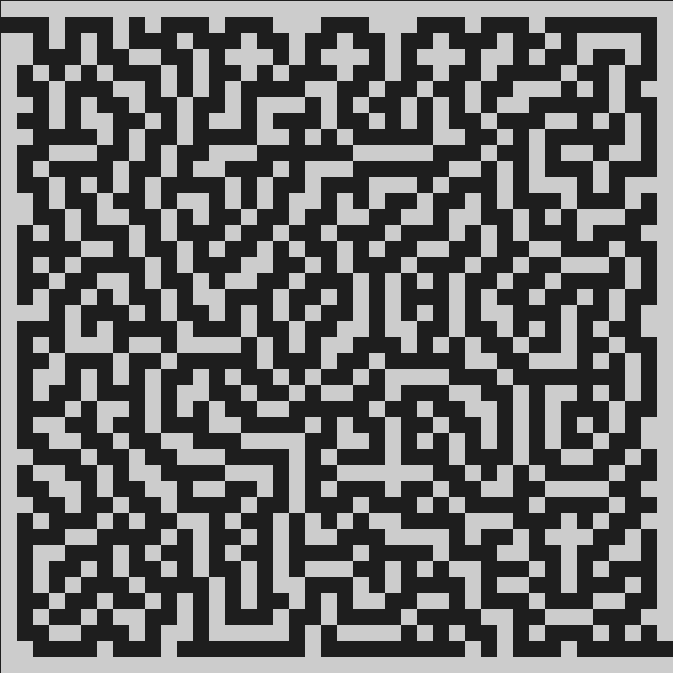
\includegraphics[width=2.5in]{1.png}
        }
        \subfigure[基于DFS的迷宫路径可视化]{
        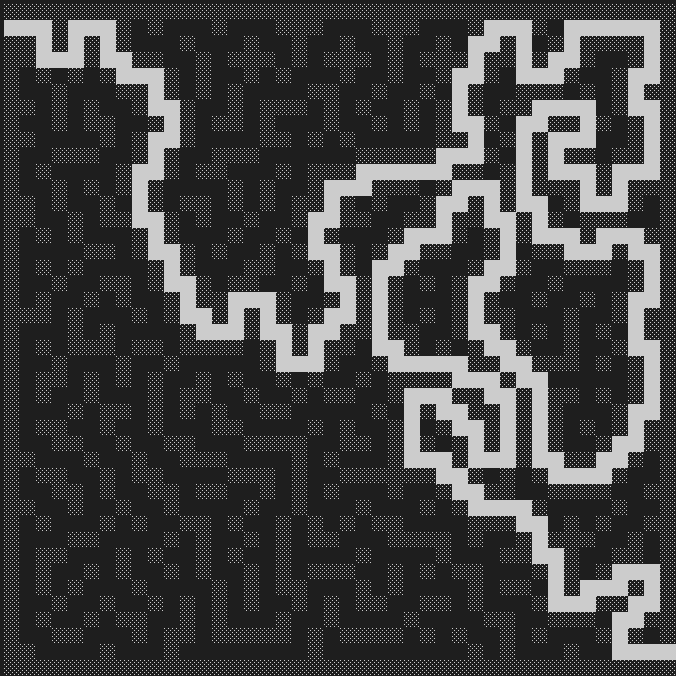
\includegraphics[width=2.5in]{2.png}
        }
        \caption{实验结果}
    \end{figure}

    由以上结果可知,实现题目的全部要求。

\subsection{时间复杂度}
$$
O(n^2)
$$
\subsection{改进方法}
可以尝试用Dijkstra算法来解决这个问题。
\section{JSON查找}

\subsection{数据结构}
\subsection{算法设计思想}
\subsection{源程序}
\subsection{测试数据及其结果}
\subsection{时间复杂度}
\subsection{改进方法}

\section{公交线路提示}
\subsection{数据结构}
\subsection{算法设计思想}
\subsection{源程序}
\subsection{测试数据及其结果}
\subsection{时间复杂度}
\subsection{改进方法}

\section{Hash表应用}
\subsection{数据结构}
\subsection{算法设计思想}
\subsection{源程序}
\subsection{测试数据及其结果}
\subsection{时间复杂度}
\subsection{改进方法}

\section{排序算法比较}
\subsection{数据结构}
\subsection{算法设计思想}
\subsection{源程序}
\subsection{测试数据及其结果}
\subsection{时间复杂度}
\subsection{改进方法}


\section{总结}
\subsection{代码行数}
\begin{table}[!h!tbp]
    \centering
  \begin{tabular*}{0.75\textwidth}{@{\extracolsep{\fill}}lcc}
      \toprule
      题目          &行数         \\
      \midrule
      区块链         &283     \\
      迷宫问题       &388     \\
      JSON查找      &$\times$    \\
      \bottomrule
  \end{tabular*}
  \end{table}
  总代码行数为:1000.
\subsection{心得体会}

\setlength{\parskip}{6pt}  %定义段间距
\vspace{4cm}
\end{document}
